\documentclass{beamer}

% To have the citation lists ordered by number.
\usepackage[nocompress]{cite}
\usepackage[utf8]{inputenc}
\usepackage{graphicx}
\usepackage[tight,TABTOPCAP]{subfigure}
\usepackage{amsmath}
\usepackage{amssymb}
\usepackage{amsfonts}
\usepackage{url}
\usepackage{xspace}

\usepackage{hyperref}

\usepackage{tikz}
\usetikzlibrary{calc}
\usetikzlibrary{shapes.symbols}
\usetikzlibrary{shapes}
\usepackage{color}

\usepackage{color}
\usepackage{listings}
\lstset{ %
language=C,                % choose the language of the code
basicstyle=\footnotesize,       % the size of the fonts that are used for the code
numbers=left,                   % where to put the line-numbers
numberstyle=\footnotesize,      % the size of the fonts that are used for the line-numbers
stepnumber=1,                   % the step between two line-numbers. If it is 1 each line will be numbered
numbersep=5pt,                  % how far the line-numbers are from the code
backgroundcolor=\color{white},  % choose the background color. You must add \usepackage{color}
showspaces=false,               % show spaces adding particular underscores
showstringspaces=false,         % underline spaces within strings
showtabs=false,                 % show tabs within strings adding particular underscores
frame=single,   		% adds a frame around the code
tabsize=2,  		% sets default tabsize to 2 spaces
captionpos=b   		% sets the caption-position to bottom
}



%%%%%%%%%% Tool Names %%%%%%%%%%%%
\newcommand{\fisch}{\textsf{Fisch}\xspace}
\newcommand{\blind}{\textsf{Blind}\xspace}
\newcommand{\hadoop}{\textsf{Hadoop}\xspace}

%%%%%%%%%% tikz macro %%%%%%%%%%%%%%%
%\sched{idx}{start}{duration}{label}
\newcommand{\sched}[4]{
  \draw[fill=blue!30] (#2/4, #1 -0.3) rectangle +(#3/4 , 0.6);
  \node at (#2/4 + #3/8, #1) {\scriptsize #4};
}
\newcommand{\schedHL}[3]{
  \draw[fill=red,opacity=0.3] (#2/4, #1 -0.3) rectangle +(#3/4 , 0.6);
}

\mode<presentation>
{
  \usetheme{Warsaw}
  %\usetheme{Frankfurt}
  % or ...

  %\setbeamercovered{transparent}
  % or whatever (possibly just delete it)
  %\setbeamertemplate{footline}[frame number]
  \useoutertheme{mysplit}
}
% Remove the navigation bar
\setbeamertemplate{navigation symbols}{}

\title[Scheduling by Abstraction Refinement]{Scheduling Large Jobs by Abstraction Refinement}

%\AtBeginSection[]
%{
%  \begin{frame}<beamer>
%    \frametitle{Outline}
%    \tableofcontents[currentsection,hideothersubsections]
%  \end{frame}
%}

\author[Damien Zufferey]{
  Thomas A.~Henzinger \and
  Vasu Singh \and
  Thomas Wies \and
  \alert{Damien Zufferey}
}

%TODO some mention of MSR in the title slide ??

\institute{ IST Austria }
\date{June 16, 2011}

%-------------------------------------------------------------------------
\begin{document}

% Title
\frame[plain]{\titlepage}

\begin{frame}
  \frametitle{Motivation (1)}
  Cloud computing gives the \emph{illusion} of $\infty$ (virtual) resources.

  \vspace{2ex}
  
  Actually there is a finite amount of (physical) resources.

  \vspace{2ex}
  
  We would like to efficiently share those resources:
  \begin{enumerate}
  \item being able to distinguish high priority (serving customer \emph{now}) from low priority (batch) requests;
  \item schedule accordingly.
  \end{enumerate}
  
  \vspace{2ex}
  
  Therefore, we should be able to \alert{plan ahead} computations.

\end{frame}

%the problem

\begin{frame}
  \frametitle{Jobs Model}
  \begin{figure}
    \centering
    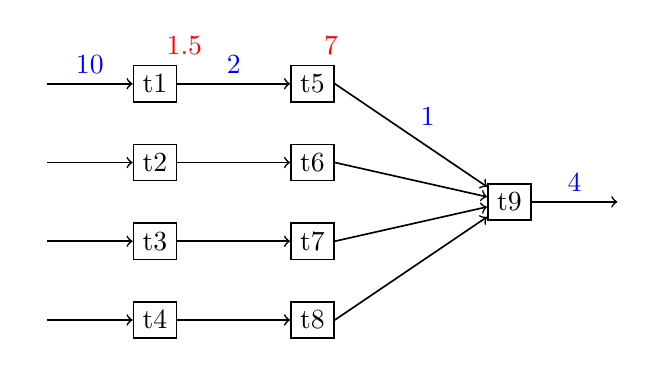
\begin{tikzpicture}[->,semithick]
      \node (d1) at (0,1.5)   {};
      \node (d2) [below of=d1]     {};
      \node (d3) [below of=d2]   {};
      \node (d4) [below of=d3]   {};
      \node[draw,label=85:\textcolor{red}{1.5}] (t1) [right=5mm, right of=d1]  {t1};
      \node[draw] (t2) [below of=t1]  {t2};
      \node[draw] (t3) [below of=t2]  {t3};
      \node[draw] (t4) [below of=t3]  {t4};
      \node[draw,label=85:\textcolor{red}{7}] (t5) [right=1cm, right of=t1]  {t5};
      \node[draw] (t6) [below of=t5]  {t6};
      \node[draw] (t7) [below of=t6]  {t7};
      \node[draw] (t8) [below of=t7]  {t8};
      \node[draw] (t9) at (6,0)    {t9};
      \node (d9) [right=5mm, right of=t9] {};
      \path (d1) edge node [above] {\textcolor{blue}{10}} (t1);
      \path (d2) edge (t2);
      \path (d3) edge (t3);
      \path (d4) edge (t4);
      \path (t1) edge node [above] {\textcolor{blue}{2}} (t5);
      \path (t2) edge (t6);
      \path (t3) edge (t7);
      \path (t4) edge (t8);
      \path (t5.east) edge node [above right] {\textcolor{blue}{1}} (t9);
      \path (t6.east) edge (t9);
      \path (t7.east) edge (t9);
      \path (t8.east) edge (t9);
      \path (t9) edge node [above] {\textcolor{blue}{4}}(d9);
    \end{tikzpicture}
  \end{figure}

  \begin{itemize}
  \item A Job is a directed acyclic task (DAG) of tasks.
  \item Node are marked with \textcolor{red}{worst case duration}.
  \item Edges are marked with \textcolor{blue}{data transfer}.
  \item duration and data can be parametric in the input.
  \end{itemize}
\end{frame}

\begin{frame}
  \frametitle{Parametric Jobs}
  \begin{figure}
    \includegraphics[scale=0.3]{parser1}
  \end{figure}
\end{frame}

\begin{frame}
  \frametitle{Infrastructure Model}

  \begin{figure}
    \centering
    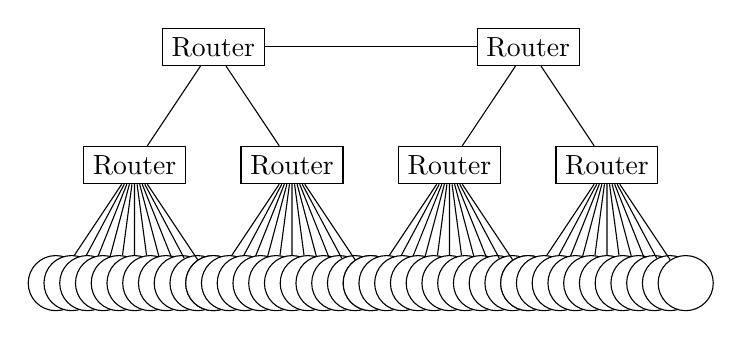
\begin{tikzpicture}
      \node[draw] (router1) at (1,3) {Router};
      \node[draw] (router2) at (5,3) {Router};
      \node[draw] (r1) at (0,1.5) {Router};
      \node[draw] (r2) at (2,1.5) {Router};
      \node[draw] (r3) at (4,1.5) {Router};
      \node[draw] (r4) at (6,1.5) {Router};
      \path (router1) edge (router2);
      \path (router1) edge (r1);
      \path (router1) edge (r2);
      \path (router2) edge (r3);
      \path (router2) edge (r4);
      \foreach \i in {0,0.2,...,2} {
        \node[draw,circle,fill=white,minimum height=7mm] (p1) at (-1 + \i, 0) {};
        \path (p1) edge (r1);
      }
      \foreach \i in {0,0.2,...,2} {
        \node[draw,circle,fill=white,minimum height=7mm] (p1) at (1 + \i, 0) {};
        \path (p1) edge (r2);
      }
      \foreach \i in {0,0.2,...,2} {
        \node[draw,circle,fill=white,minimum height=7mm] (p1) at (3 + \i, 0) {};
        \path (p1) edge (r3);
      }
      \foreach \i in {0,0.2,...,2} {
        \node[draw,circle,fill=white,minimum height=7mm] (p1) at (5 + \i, 0) {};
        \path (p1) edge (r4);
      }
    \end{tikzpicture}
  \end{figure}

  Datacentre as a tree-like graph:
  \begin{itemize}
  \item internal nodes are router;
  \item leaves are compute nodes (computation speed);
  \item edges specifies the bandwidth.
  \end{itemize}

\end{frame}

\begin{frame}
  \frametitle{Schedule}

  \begin{center}
  A relation between tasks, nodes, and time.
  \end{center}
  
  \begin{figure}
  \centering
  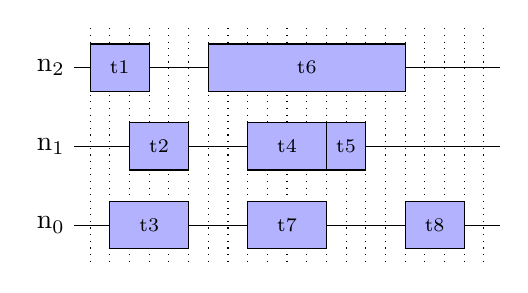
\begin{tikzpicture}
      \foreach \i in {0,1,...,2} {
        \draw (-0.2,\i) -- (5.2,\i);
        \node at (-0.5,\i) {n$_\i$};
      }
      \foreach \i in {0,1,...,20} {
        \draw[dotted] (\i/4,2.5) -- (\i/4,-0.5);
      }

      \sched{2}{0}{3}{t1}
      \sched{2}{6}{10}{t6}
      
      \sched{1}{2}{3}{t2}
      \sched{1}{8}{4}{t4}
      \sched{1}{12}{2}{t5}

      \sched{0}{1}{4}{t3}
      \sched{0}{8}{4}{t7}
      \sched{0}{16}{3}{t8}
  \end{tikzpicture}
  \end{figure}


\end{frame}


\begin{frame}
  \frametitle{Problem: the scale}
  \begin{minipage}[t]{0.45\linewidth}
    On the infrastructure side:
    \begin{figure}
    \centering
    \includegraphics[scale=0.3]{beautiful-datacenter-wiring14.jpg}
    \end{figure}
  \end{minipage}
  \hfill
  \begin{minipage}[t]{0.45\linewidth}
    On the job side:
    \begin{figure}
    \centering
    \includegraphics[scale=0.3]{large_job}
    \end{figure}
  \end{minipage}

  \vspace{1cm}

  Given the scale, people have been using dynamic scheduling.
\end{frame}

\begin{frame}
  \frametitle{Example: \hadoop MapReduce engine}
  \begin{figure}
    \centering
    \includegraphics[scale=0.5]{hadoop}
  \end{figure}
\end{frame}

\begin{frame}
  \frametitle{Motivation (2)}

  Dynamic Scheduling: use work queues, priorities, but limited.

  \vspace{2ex}
  
  Without knowledge of jobs, this is the best you can do.

  \vspace{1cm}
  
  We need to ask the user submitting a job for:
  \begin{itemize}
  \item what kind of resources the job requires;
  \item a deadline/priority for the job.
  \end{itemize}

  \vspace{2ex}
  
  In exchange we can give him an expected completion time.

\end{frame}

\begin{frame}
  \frametitle{Giving incentive to plan in advance}

  The scheduler returns not one but many possible schedules with different finish times.

  Use a pricing model to associate a cost to the schedules.

  Include the ``scheduling difficulty'' in the cost, give a discount to schedule with later finish time.

  \begin{figure}
    \includegraphics[scale=0.3]{price_curve}
  \end{figure}

  Problem: static scheduling is \emph{hard}.

  Only possible if the scheduler can handle the work load.

\end{frame}

\begin{frame}
  \frametitle{Static scheduling:}

  Computing optimal schedule: NP-hard
  
  \vspace{10pt}

  Heuristics (Greedy, deadline division etc.): $|J|\cdot|C|$

  \vspace{10pt}

  With 1000 tasks job and 200 nodes cloud, a greedy scheduler takes up to 5 minutes!
   
  \vspace{10pt}

  To do better we should try to solve only a simplified problem.
\end{frame}

\begin{frame}
  \frametitle{Core idea:}
  Assumption: job and infrastructure \alert{regularity} 

  \vspace{1ex}

  Idea: regularity makes large scale scheduling feasible

  \vspace{1ex}

  How: Using abstraction techniques

  \vspace{1ex}

  \begin{itemize}
  \item Over-approximate the resources needed by the job $J$ to get $J^\#$.
  \item Under-approximate the available resources for the cloud $C$ to get $C^\#$.
  \item Get a schedule for $(J^\#,C^\#)$ and use it to construct a schedule for $(J,C)$.
  \end{itemize}
  
  \vspace{1ex}

  Approximation is done in order to introduce regularity (symmetry).
  
  Symmetry can be captured using multiplicity.

  Over-/Under-approximation guarantees the existence of a schedule.

\end{frame}


\begin{frame}
  \frametitle{Scheduling using abstraction refinement}

  \begin{figure}
    \includegraphics[scale=0.35]{abs_scheduling}
  \end{figure}

  When to refine: not good enough (utilisation, makespan).

\end{frame}

\begin{frame}
  \frametitle{Abstraction for jobs:}

  Group independent tasks as per a topological sort.
  Merge them into an abstract task.

  \begin{figure}
    \centering
    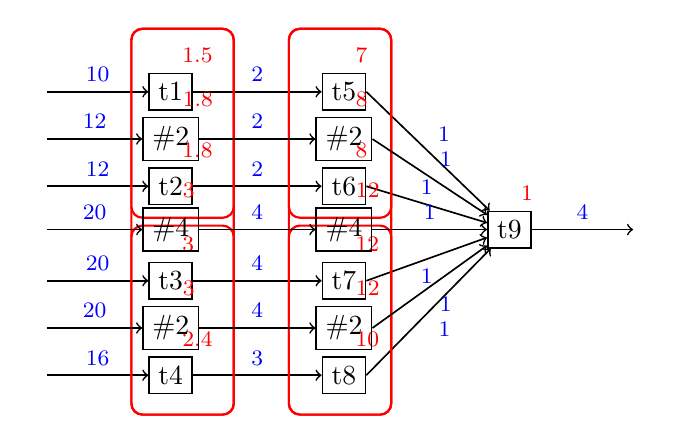
\begin{tikzpicture}[->,semithick, node distance=12mm]
      \node[draw,label=85:\textcolor{red}{\footnotesize 1}] (t9) at (6,-0.25)    {t9};
      \node (d9) [right=5mm, right of=t9] {};
      \path (t9) edge node [above] {\textcolor{blue}{\footnotesize 4}}(d9);
      \visible<1,2,4>{
      \node (d1) at (0,1.5)     {};
      \node (d2) [below of=d1]  {};
      \node (d3) [below of=d2]  {};
      \node (d4) [below of=d3]  {};
      \node[draw,label=85:\textcolor{red}{\footnotesize 1.5}] (t1) [right=5mm, right of=d1]  {t1};
      \node[draw,label=85:\textcolor{red}{\footnotesize 1.8}] (t2) [below of=t1]  {t2};
      \node[draw,label=85:\textcolor{red}{\footnotesize   3}] (t3) [below of=t2]  {t3};
      \node[draw,label=85:\textcolor{red}{\footnotesize 2.4}] (t4) [below of=t3]  {t4};
      \node[draw,label=85:\textcolor{red}{\footnotesize  7}] (t5) [right=1cm, right of=t1]  {t5};
      \node[draw,label=85:\textcolor{red}{\footnotesize  8}] (t6) [below of=t5]  {t6};
      \node[draw,label=85:\textcolor{red}{\footnotesize 12}] (t7) [below of=t6]  {t7};
      \node[draw,label=85:\textcolor{red}{\footnotesize 10}] (t8) [below of=t7]  {t8};
      \path (d1) edge node [above] {\textcolor{blue}{\footnotesize 10}} (t1);
      \path (d2) edge node [above] {\textcolor{blue}{\footnotesize 12}} (t2);
      \path (d3) edge node [above] {\textcolor{blue}{\footnotesize 20}} (t3);
      \path (d4) edge node [above] {\textcolor{blue}{\footnotesize 16}} (t4);
      \path (t1) edge node [above] {\textcolor{blue}{\footnotesize 2}} (t5);
      \path (t2) edge node [above] {\textcolor{blue}{\footnotesize 2}} (t6);
      \path (t3) edge node [above] {\textcolor{blue}{\footnotesize 4}} (t7);
      \path (t4) edge node [above] {\textcolor{blue}{\footnotesize 3}} (t8);
      \path (t5.east) edge node [above right] {\textcolor{blue}{\footnotesize 1}} (t9);
      \path (t6.east) edge node [above ] {\textcolor{blue}{\footnotesize 1}} (t9);
      \path (t7.east) edge node [below ] {\textcolor{blue}{\footnotesize 1}} (t9);
      \path (t8.east) edge node [below right] {\textcolor{blue}{\footnotesize 1}} (t9);
      \visible<2>{
        \draw[rounded corners,red,thick] (1.2,2.3) rectangle +(1.3,-4.9);
        \draw[rounded corners,red,thick] (3.2,2.3) rectangle +(1.3,-4.9);
      }
      \visible<4>{
        \draw[rounded corners,red,thick] (1.2,2.3) rectangle +(1.3,-2.4);
        \draw[rounded corners,red,thick] (1.2,-0.2) rectangle +(1.3,-2.4);
        \draw[rounded corners,red,thick] (3.2,2.3) rectangle +(1.3,-2.4);
        \draw[rounded corners,red,thick] (3.2,-0.2) rectangle +(1.3,-2.4);
      }
      }
      \visible<3>{
      \node (d22) at (0,-0.25)     {};
      \node[draw,label=85:\textcolor{red}{\footnotesize 3}] (t22) [right=5mm, right of=d22]  {\#4};
      \node[draw,label=85:\textcolor{red}{\footnotesize  12}] (t62) [right=1cm, right of=t22]  {\#4};
      \path (d22) edge node [above] {\textcolor{blue}{\footnotesize 20}} (t22);
      \path (t22) edge node [above] {\textcolor{blue}{\footnotesize 4}} (t62);
      \path (t62.east) edge node [above] {\textcolor{blue}{\footnotesize 1}} (t9);
      }
      \visible<5>{
      \node (d12) at (0,0.9)     {};
      \node[draw,label=85:\textcolor{red}{\footnotesize 1.8}] (t12) [right=5mm, right of=d12]  {\#2};
      \node[draw,label=85:\textcolor{red}{\footnotesize  8}] (t52) [right=1cm, right of=t12]  {\#2};
      \path (d12) edge node [above] {\textcolor{blue}{\footnotesize 12}} (t12);
      \path (t12) edge node [above] {\textcolor{blue}{\footnotesize 2}} (t52);
      \path (t52.east) edge node [above right] {\textcolor{blue}{\footnotesize 1}} (t9);
      \node (d32) at (0,-1.5)     {};
      \node[draw,label=85:\textcolor{red}{\footnotesize 3}] (t32) [right=5mm, right of=d32]  {\#2};
      \node[draw,label=85:\textcolor{red}{\footnotesize 12}] (t72) [right=1cm, right of=t32]  {\#2};
      \path (d32) edge node [above] {\textcolor{blue}{\footnotesize 20}} (t32);
      \path (t32) edge node [above] {\textcolor{blue}{\footnotesize 4}} (t72);
      \path (t72.east) edge node [below right] {\textcolor{blue}{\footnotesize 1}} (t9);
      }
    \end{tikzpicture}
  \end{figure}

  Decide when to merge based on similarity.

  Two tasks with duration $d_1,d_2$ are $X$-similar iff $1/X \leq d_1/d_2\leq X$.

\end{frame}

\begin{frame}
  \frametitle{Datacentre abstraction}
  
  Rack abstraction: Create an abstract node for a group of nodes on a rack

  \begin{figure}
    \centering
    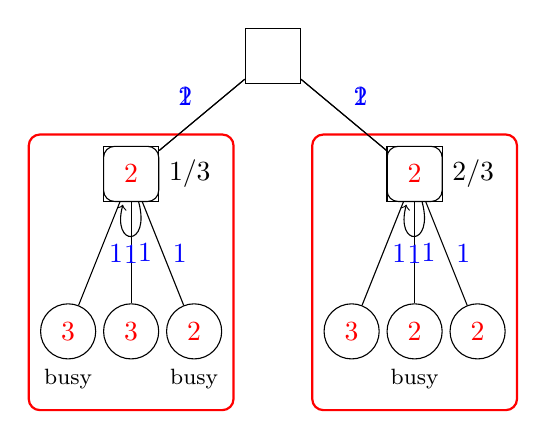
\begin{tikzpicture}[
        router/.style={draw, rectangle,minimum width=7mm, minimum height=7mm},
        machine/.style={draw, circle, minimum width=7mm, minimum height=7mm},
        abstract/.style={draw, rectangle, rounded corners, minimum width=7mm, minimum height=7mm}
      ]

    \node[router] (r1) at (0,0.5) {};

    \visible<1,2>{
    \node[router] (r2) at (-1.8,-1) {};
    \node[router] (r3) at (1.8,-1) {};

    \node[machine,label=below:{\footnotesize busy}] (m1) at (-2.6,-3) {\textcolor{red}{3}};
    \node[machine] (m2) at (-1.8,-3) {\textcolor{red}{3}};
    \node[machine,label=below:{\footnotesize busy}] (m3) at (-1,-3) {\textcolor{red}{2}};
    \node[machine] (m4) at (1,-3) {\textcolor{red}{3}};
    \node[machine,label=below:{\footnotesize busy}] (m5) at (1.8,-3) {\textcolor{red}{2}};
    \node[machine] (m6) at (2.6,-3) {\textcolor{red}{2}};
    \path (r1) edge node [above left] {\textcolor{blue}{2}} (r2);
    \path (r1) edge node [above right] {\textcolor{blue}{2}} (r3);
    \path (r2) edge node [right] {\textcolor{blue}{1}} (m1);
    \path (r2) edge node [right=-1pt] {\textcolor{blue}{1}} (m2);
    \path (r2) edge node [right] {\textcolor{blue}{1}} (m3);
    \path (r3) edge node [right] {\textcolor{blue}{1}} (m4);
    \path (r3) edge node [right=-1pt] {\textcolor{blue}{1}} (m5);
    \path (r3) edge node [right] {\textcolor{blue}{1}} (m6);
    }
    
    \visible<2>{
      \draw[rounded corners,red,thick] (-3.1,-0.5) rectangle +(2.6,-3.5);
      \draw[rounded corners,red,thick] (0.5,-0.5) rectangle +(2.6,-3.5);
    }

    \visible<3>{
    \node[abstract,label=right:{$1/3$}] at (-1.8,-1) (l1) {\textcolor{red}{2}};
    \node[abstract,label=right:{$2/3$}] (l2) at (1.8,-1) {\textcolor{red}{2}};
    \draw (l1) edge [loop below] node {\textcolor{blue}{1}} (l1);
    \draw (l2) edge [loop below] node {\textcolor{blue}{1}} (l2);
    \path (r1) edge node [above left] {\textcolor{blue}{1}} (l1);
    \path (r1) edge node [above right] {\textcolor{blue}{1}} (l2);
    }

    \end{tikzpicture}

  \end{figure}

\end{frame}

\begin{frame}
  \frametitle{Two AR scheduler}
  
  {\large\bf
  \fisch: Free intervals scheduler
  }

  \vspace{10pt}

  fixed datacentre abstraction,\\
  refines the job abstraction.

  \vspace{2cm}

  {\large\bf
  \blind: Buddy-list in datacentre
  }

  \vspace{10pt}

  fixed job abstraction,\\
  refines the datacentre abstraction.

\end{frame}

\begin{frame}<1-8>
  \frametitle{\fisch: Free intervals scheduler}
  Build an index (search engine) to track only the free intervals.

  \begin{figure}
  \centering
  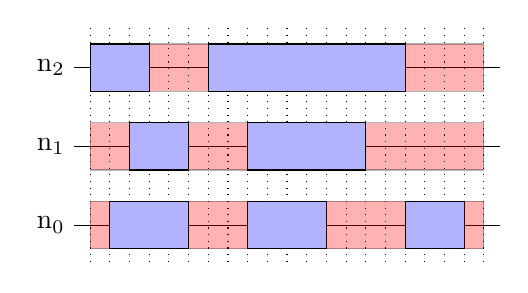
\begin{tikzpicture}
      \foreach \i in {0,1,...,2} {
        \draw (-0.2,\i) -- (5.2,\i);
        \node at (-0.5,\i) {n$_\i$};
      }
      \foreach \i in {0,1,...,20} {
        \draw[dotted] (\i/4,2.5) -- (\i/4,-0.5);
      }

      \visible<1>{
      \sched{2}{0}{3}{t1}
      \sched{2}{6}{10}{t6}
      \sched{1}{2}{3}{t2}
      \sched{1}{8}{4}{t4}
      \sched{1}{12}{2}{t5}
      \sched{0}{1}{4}{t3}
      \sched{0}{8}{4}{t7}
      \sched{0}{16}{3}{t8}
      }
      \visible<2->{
      \sched{2}{0}{3}{}
      \sched{2}{6}{10}{}
      \sched{1}{2}{3}{}
      \sched{1}{8}{6}{}
      \sched{0}{1}{4}{}
      \sched{0}{8}{4}{}
      \sched{0}{16}{3}{}
      }

      \visible<3>{\schedHL{0}{0}{1}}
      \visible<4>{\schedHL{1}{0}{2}}
      \visible<5>{\schedHL{2}{3}{3}}
      \visible<5>{\schedHL{0}{5}{3}}
      \visible<5>{\schedHL{1}{5}{3}}
      \visible<6>{\schedHL{0}{12}{4}}
      \visible<7>{\schedHL{0}{19}{1}}
      \visible<7>{\schedHL{1}{14}{6}}
      \visible<7>{\schedHL{2}{16}{4}}
  \end{tikzpicture}
  \end{figure}

  Index of the free intervals (computed at the rack level):

  \vspace{1ex}

  {\small
  \begin{tabular}{ccl}
    1  & : & \temporal<3>{ }{ \alert{(n$_0$,0)} }{ (n$_0$,0) } \\
    2  & : & \temporal<4>{ }{ \alert{(n$_1$,0)} }{ (n$_1$,0) } \\
    3  & : & \temporal<5>{ }{ \alert{(n$_2$,3), (n$_0$,5), (n$_1$,5)} }{ (n$_2$,3), (n$_0$,5), (n$_1$,5) } \\
    4  & : & \temporal<6>{ }{ \alert{(n$_0$,12)} }{ (n$_0$,12) } \\
    \_ & : & \temporal<7>{ }{ \alert{(n$_1$,14), (n$_2$,16), (n$_0$,19)} }{ (n$_1$,14), (n$_2$,16), (n$_0$,19) }
  \end{tabular}
  }

  \vspace{2ex}

  Starts with an $X$-similar job abstraction where $X=\infty$

  Refinement lowers the $X$

\end{frame}

\begin{frame}
  \frametitle{\blind: Buddy-list in datacentre}
  buddy-list (garbage collection) principle to group machines.

  \begin{figure}
    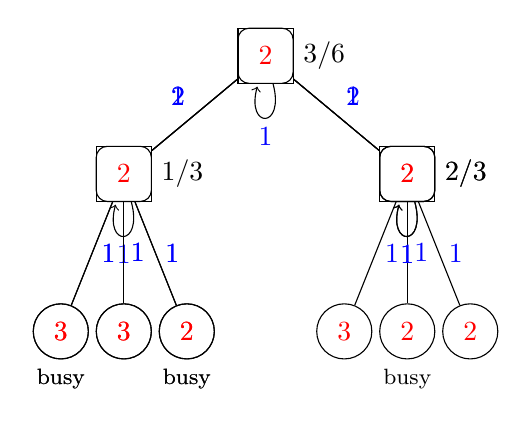
\begin{tikzpicture}[
        router/.style={draw, rectangle,minimum width=7mm, minimum height=7mm},
        machine/.style={draw, circle, minimum width=7mm, minimum height=7mm},
        abstract/.style={draw, rectangle, rounded corners, minimum width=7mm, minimum height=7mm}
      ]


    \visible<1,6>{
    \node[router] (r1) at (0,0.5) {};
    \node[router] (r2) at (-1.8,-1) {};
    \node[router] (r3) at (1.8,-1) {};

    \node[machine,label=below:{\footnotesize busy}] (m1) at (-2.6,-3) {\textcolor{red}{3}};
    \node[machine] (m2) at (-1.8,-3) {\textcolor{red}{3}};
    \node[machine,label=below:{\footnotesize busy}] (m3) at (-1,-3) {\textcolor{red}{2}};
    \node[machine] (m4) at (1,-3) {\textcolor{red}{3}};
    \node[machine,label=below:{\footnotesize busy}] (m5) at (1.8,-3) {\textcolor{red}{2}};
    \node[machine] (m6) at (2.6,-3) {\textcolor{red}{2}};
    \path (r1) edge node [above left] {\textcolor{blue}{2}} (r2);
    \path (r1) edge node [above right] {\textcolor{blue}{2}} (r3);
    \path (r2) edge node [right] {\textcolor{blue}{1}} (m1);
    \path (r2) edge node [right=-1pt] {\textcolor{blue}{1}} (m2);
    \path (r2) edge node [right] {\textcolor{blue}{1}} (m3);
    \path (r3) edge node [right] {\textcolor{blue}{1}} (m4);
    \path (r3) edge node [right=-1pt] {\textcolor{blue}{1}} (m5);
    \path (r3) edge node [right] {\textcolor{blue}{1}} (m6);
    }
    
    \visible<2,4>{
    \node[router] (r1) at (0,0.5) {};
    \node[abstract,label=right:{$1/3$}] at (-1.8,-1) (l1) {\textcolor{red}{2}};
    \node[abstract,label=right:{$2/3$}] (l2) at (1.8,-1) {\textcolor{red}{2}};
    \draw (l1) edge [loop below] node {\textcolor{blue}{1}} (l1);
    \draw (l2) edge [loop below] node {\textcolor{blue}{1}} (l2);
    \path (r1) edge node [above left] {\textcolor{blue}{1}} (l1);
    \path (r1) edge node [above right] {\textcolor{blue}{1}} (l2);
    }

    \visible<3>{
    \node[abstract,label=right:{$3/6$}] (r1) at (0,0.5) {\textcolor{red}{2}};
    \draw (r1) edge [loop below] node {\textcolor{blue}{1}} (r1);
    }
    
    \visible<5>{
    \node[router] (r1) at (0,0.5) {};
    \node[router] (r2) at (-1.8,-1) {};
    \node[abstract,label=right:{$2/3$}] (l2) at (1.8,-1) {\textcolor{red}{2}};
    \draw (l2) edge [loop below] node {\textcolor{blue}{1}} (l2);
    \path (r1) edge node [above right] {\textcolor{blue}{1}} (l2);
    \node[machine,label=below:{\footnotesize busy}] (m1) at (-2.6,-3) {\textcolor{red}{3}};
    \node[machine] (m2) at (-1.8,-3) {\textcolor{red}{3}};
    \node[machine,label=below:{\footnotesize busy}] (m3) at (-1,-3) {\textcolor{red}{2}};
    \path (r1) edge node [above left] {\textcolor{blue}{2}} (r2);
    \path (r2) edge node [right] {\textcolor{blue}{1}} (m1);
    \path (r2) edge node [right=-1pt] {\textcolor{blue}{1}} (m2);
    \path (r2) edge node [right] {\textcolor{blue}{1}} (m3);
    }
    
    \end{tikzpicture}
  \end{figure}

  Uses utilisation as quality measure to decide when to refine a node.

\end{frame}

\begin{frame}
  \frametitle{ Infrastructure Refinement: a race to the bottom ?}
  
  If we keep on refining we eventually get to the concrete system.
  
  Thus, an abstraction would only provide transient gain.

  \vspace{1ex}

  We also need to \alert{coarsen} the abstraction.

  \vspace{1ex}

  Caveat: for a given abstraction there are concrete schedules with no corresponding abstract schedules.

  \vspace{1ex}

  Fortunately, time is on our side.
  Tasks scheduled at a finer level of abstraction will eventually be executed.
  However, there is a transition period with two abstractions levels.

\end{frame}

\begin{frame}
  \frametitle{ Allocation on an abstract node }
  
  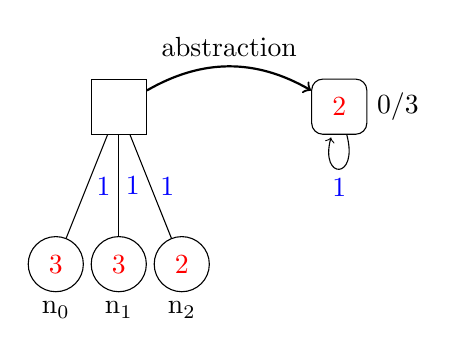
\begin{tikzpicture}[
      router/.style={draw, rectangle,minimum width=7mm, minimum height=7mm},
      machine/.style={draw, circle, minimum width=7mm, minimum height=7mm},
      abstract/.style={draw, rectangle, rounded corners, minimum width=7mm, minimum height=7mm}
    ]

    \node[router] (r2) at (-1.8,-1) {};
    \node[machine,label=below:{n$_0$}] (m1) at (-2.6,-3) {\textcolor{red}{3}};
    \node[machine,label=below:{n$_1$}] (m2) at (-1.8,-3) {\textcolor{red}{3}};
    \node[machine,label=below:{n$_2$}] (m3) at (-1,-3) {\textcolor{red}{2}};
    \path (r2) edge node [right] {\textcolor{blue}{1}} (m1);
    \path (r2) edge node [right=-1pt] {\textcolor{blue}{1}} (m2);
    \path (r2) edge node [right] {\textcolor{blue}{1}} (m3);

    \node[abstract,label=right:{$0/3$}] (r1) at (1,-1) {\textcolor{red}{2}};
    \draw (r1) edge [loop below] node {\textcolor{blue}{1}} (r1);

    \path (r2) edge [->,bend left,thick] node [above] {abstraction} (r1);
  \end{tikzpicture}
  \hfill
  \begin{minipage}[b]{0.4\linewidth}
  Schedule:

  \vspace{1ex}

  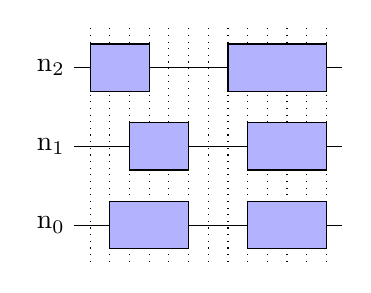
\begin{tikzpicture}
      \foreach \i in {0,1,...,2} {
        \draw (-0.2,\i) -- (3.2,\i);
        \node at (-0.5,\i) {n$_\i$};
      }
      \foreach \i in {0,1,...,12} {
        \draw[dotted] (\i/4,2.5) -- (\i/4,-0.5);
      }
      \sched{2}{0}{3}{}
      \sched{2}{7}{5}{}
      \sched{1}{2}{3}{}
      \sched{1}{8}{4}{}
      \sched{0}{1}{4}{}
      \sched{0}{8}{4}{}
  \end{tikzpicture}
  \end{minipage}


  New request: 2 nodes for 3 units of time.

  \vspace{1ex}

  \visible<2->{
  Events: {\small (0,-1), (1,-1), (2,-1), (3,+1), (5,+2), (7,-1), (8,-2), (12,+3)}
  }

  \vspace{1ex}

  \visible<3>{
  \begin{minipage}{0.3\linewidth}
  Traverses the events and shifts the allocations by -3+$\epsilon$
  \end{minipage}
  \begin{minipage}{0.37\linewidth}
  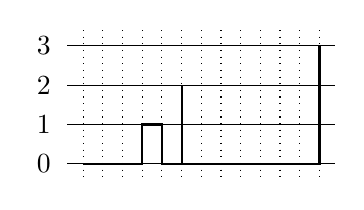
\begin{tikzpicture}
      \foreach \i in {0,1,...,3} {
        \draw (-0.2,\i/2) -- (3.2,\i/2);
        \node at (-0.5,\i/2) {\i};
      }
      \foreach \i in {0,1,...,12} {
        \draw[dotted] (\i/4,1.7) -- (\i/4,-0.2);
      }
      \path[draw, thick] (0,0) -- (3/4,0) -- (3/4,1/2) -- (4/4,1/2) -- (4/4,0) -- (5/4,0) -- (5/4,1) -- (5/4,0) -- (12/4,0) -- (12/4,3/2);
  \end{tikzpicture}
  \end{minipage}
  \begin{minipage}{0.3\linewidth}
  Guarantees that there is two free nodes at 5, but \alert{does not tell which ones}
  \end{minipage}
  }

  
\end{frame}

\begin{frame}
  \frametitle{ Experiments, part 1: simulation }

  \begin{minipage}[t]{0.4\linewidth}
    datacenter:
    \begin{figure}
    \centering
    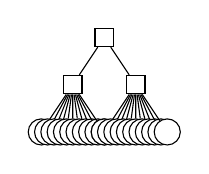
\begin{tikzpicture}[scale=0.4]
      \node[draw] (router1) at (1,3) {};
      \node[draw] (r1) at (0,1.5) {};
      \node[draw] (r2) at (2,1.5) {};
      \path (router1) edge (r1);
      \path (router1) edge (r2);
      \foreach \i in {0,0.2,...,2} {
        \node[draw,circle,fill=white] (p1) at (-1 + \i, 0) {};
        \path (p1) edge (r1);
      }
      \foreach \i in {0,0.2,...,2} {
        \node[draw,circle,fill=white] (p1) at (1 + \i, 0) {};
        \path (p1) edge (r2);
      }
    \end{tikzpicture}

    \end{figure}

    2-tier datacenter
    
    Half of the nodes: speed x,
    
    Other half: speed 1.5 x

  \end{minipage}
  \hfill
  \begin{minipage}[t]{0.55\linewidth}
    On the job side:
    \begin{figure}
    \centering
    \includegraphics[scale=0.4]{all_jobs}
    \end{figure}
  \end{minipage}

\end{frame}

\begin{frame}
  \frametitle{ Experiments: the cost of abstraction }
  We then compare \fisch and \blind to a concrete greedy scheduler (baseline) on a sequence of 100 jobs (10-5000 tasks each).
  Latency is given per tasks.

  \begin{figure}

    \begin{minipage}{0.55\linewidth}
    \begin{tabular}{l|cc}
    Scheduler & Latency & Utilization \\
              & (ms)    &  \\
    \hline
    Baseline  & 293     & 96 \% \\
    \fisch    & 0.27    & 92 \% \\
    \blind    & 0.16    & 91 \%
    \end{tabular}
    \vfill
    \subfigure[Baseline]{ \includegraphics[scale=0.3]{base_util} }
    \end{minipage}
    \begin{minipage}{0.43\linewidth}
    \subfigure[\fisch]{ \includegraphics[scale=0.3]{fisch_util} }
    \subfigure[\blind]{ \includegraphics[scale=0.3]{blind_util} }
    \end{minipage}
  \end{figure}
\end{frame}

\begin{frame}
  \frametitle{ Experiments: scaling}
    \begin{minipage}{0.3\linewidth}
    \begin{tabular}{ll}
    C1: & 2000 nodes,\\
        & 20 per rack\\
    C2: & 1600 nodes,\\
        & 40 per rack\\
    C3: & 4000 nodes,\\
        & 20 per rack\\
    C4: & 8000 nodes,\\
        & 20 per rack\\
    C6: & 1000 nodes,\\
        & 500 per rack
    \end{tabular}
    \end{minipage}
    \begin{minipage}{0.65\linewidth}
    \includegraphics[scale=0.7]{latency_fisch}

    \includegraphics[scale=0.7]{latency_blind}
    \end{minipage}
\end{frame}

\begin{frame}
  \frametitle{ Experiments, part 2: real world }

  Caution: static scheduling alone will not work.
  \begin{itemize}
  \item Task duration are conservative estimates;
  \item Variability of the performance of the compute node.
  \end{itemize}
  We use static scheduling with backfilling.

  \hfill

  Job:
  \begin{itemize}
  \item The jobs are MapReduce jobs doing image transformation.
  \item Mapper: 8.1 seconds on average, estimate is 40 seconds
  \item Reducer: Identity operation
  \end{itemize}

  \hfill

  Infrastructure:
  \begin{itemize}
  \item Hadoop streaming version 0.19.0
  \item Amazon EC2 m1.xlarge instances (15GB RAM, 4 cores)
  \item Number of mappers = 50 * number of instances
  \end{itemize}

\end{frame}

\begin{frame}
  \frametitle{ Experiments: compared to \hadoop }

  \begin{figure}
    \includegraphics[scale=0.4]{comp_hadoop_1}
    \hspace{1ex}
    \includegraphics[scale=0.4]{comp_hadoop_2}
  \end{figure}
  
  \vfill

  Observations:
  \begin{itemize}
  \item The Hadoop framework requires large runtime overhead: results in slowdown of the job execution.
  \item Static scheduling allows to prefetch data, whereas dynamic scheduling does not
  \end{itemize}

\end{frame}

\begin{frame}
  \frametitle{Conclusion}

  There is an opportunity to apply methods developed to solve computationally hard problem in verification to other area.
  While preserving a solid theoretical basis.

  \hfill

  \begin{center}
  \huge
  Questions ?
  \end{center}
\end{frame}


\end{document}
